% !TEX root = Monografia Mestrado.tex

\chapter{ISO 29110}

\section{Divisão da \iso}

A \iso é dividida em cinco partes, sendo uma visão global, dois perfis (\textit{Framework} e taxonomia e especificações de perfis das VSE) e dois guias (guia de avaliação e guia de gestão e engenharia). Sua composição pode ser visualizada na Figura \ref{fig:serie:iso}.

\begin{figure}[!h]
\centering
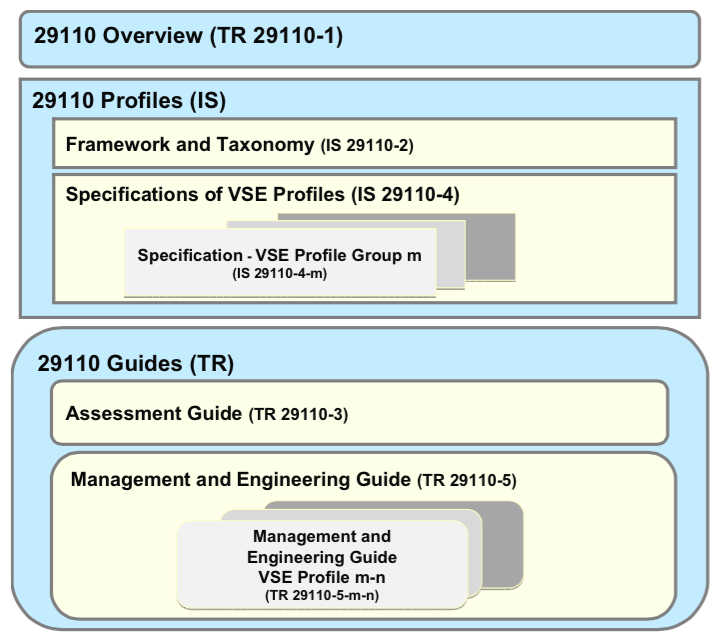
\includegraphics[scale=0.4]{figuras/serie_iso.png}
\caption{Série \iso \cite[pág. 7]{iso}}
\label{fig:serie:iso}
\end{figure}

O guia de gestão e engenharia oferece às VSE processos de \gp e \dsw que, de acordo com \cite{iso}, fazem com que os desenvolvedores ganhem benefícios através dos seguintes aspectos alcançados:

\begin{itemize}

\item Um conjunto de requisitos de projeto e produtos esperados é entregue ao cliente;

\item Um processo disciplinado de gestão que oferece visibilidade do projeto e ações corretivas para problemas e desvios de projeto é realizado;

\item Um processo sistemático e disciplinado de desenvolvimento de \sw que satisfaça as necessidades do cliente e assegure a qualidade do produto é seguido.

\end{itemize}

O guia também cita algumas condiç	ões iniciais para que a VSE possa utilizá-lo \citep{iso}:

\begin{itemize}

\item Documentação da Declaração de Trabalho do projeto;

\item Realização do estudo de viabilidade do projeto, antes do seu início;

\item Atribuição e treinamento da equipe de projeto, incluindo o gerente de projeto;

\item Disponibilidade de bens, serviços e infraestrutura para se iniciar o projeto.

\end{itemize}

Os processos de \gp e \dsw são interrelacionados, sendo a entrada do primeiro a \dt e saída do último a \swcfg, conforme pode ser observado na Figura \ref{fig:gp:dsw}. 

A \gp está ligada ao estabelecimento e controle das tarefas para se alcançar os objetivos do projeto em termos de qualidade, tempo e custo. O \dsw está relacionado às atividades de construção, integração e testes de \sw.

\begin{figure}[!h]
\centering
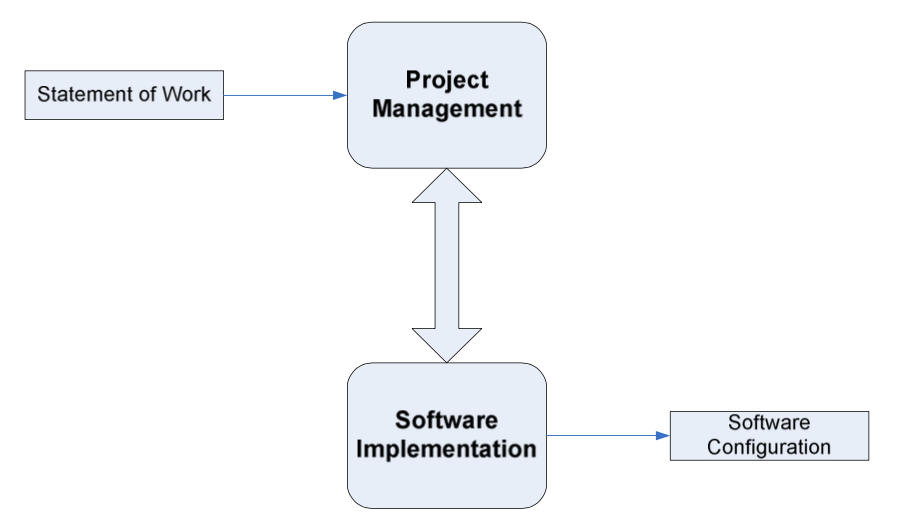
\includegraphics[scale=0.3]{figuras/gp_desenv_sw.png}
\caption{Processos básicos \cite[pág. 12]{iso}}
\label{fig:gp:dsw}
\end{figure}

\section{\gp}

De acordo com \cite{iso}, os objetivos deste processo são:

\begin{itemize}

\item[PM.O1] O \ppj é desenvolvido de acordo com a \dt e é revisado e aceito pelo cliente. As tarefas e recursos necessários para completar o trabalho são quantificados e estimados.

\item[PM.02] O progresso do projeto é monitorado em relação ao \ppj e registrado no \prog. Correções para remediar problemas e desvios do plano são tomadas quando os objetivos do projeto não são alcançados. O fechamento do projeto é realizado para se conseguir o aceite do cliente documentado no \aceite.

\item[PM.03] A \muda é abordada através de sua recepção e análise. Mudanças aos requisitos de \sw são avaliadas em custo, cronograma e impacto técnico.

\item[PM.O4] Reuniões de revisão são realizadas com a equipe de trabalho e o cliente. Acertos são registrados e rastreados.

\item[PM.O5] Riscos são identificados conforme aparecem e durante a condução do projeto.

\item[PM.O6] Uma \vcs de \sw é desenvolvida. Itens da \swcfg são identificados, definidos e incluídos em uma \bline. Modificações e entregas de um item são controladas e disponibilizadas ao cliente e equipe de trabalho. O armazenamento, manuseio e entrega dos itens são controlados.

\item[PM.O7] A \qsw é realizada para garantir que os produtos de trabalho e processos obedeçam ao \ppj e \req.

\end{itemize}

Cada um destes objetivos pode ser alcançado através de uma série de processos que, por sua vez, irão gerar vários documentos de apoio. Os processos e o fluxo de informação que percorre estes processos podem ser resumidos na Figura \ref{fig:gp:diagr}.

\begin{figure}[!h]
\centering
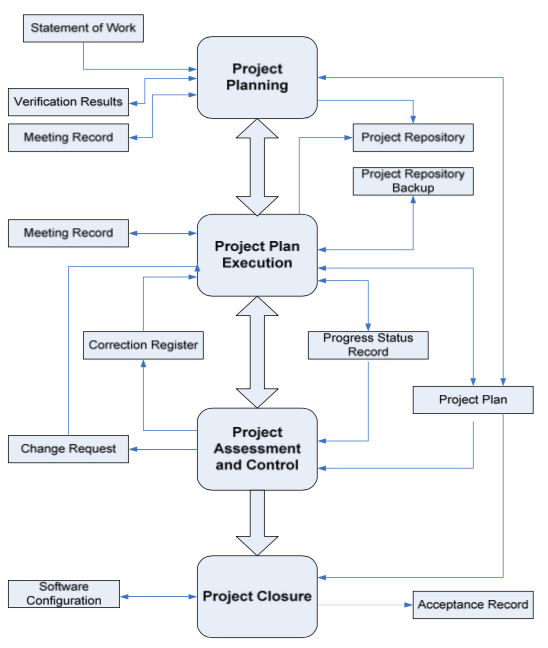
\includegraphics[scale=0.5]{figuras/gp_diagr.png}
\caption{Diagrama do processo de \gp \cite[pág. 12]{iso}}
\label{fig:gp:diagr}
\end{figure}

\section{\dsw}

De acordo com \cite{iso}, os objetivos deste processo são:

\begin{itemize}

\item[SI.O1] As tarefas das atividades são feitas através da realização do \ppj corrente.

\item[SI.02] Os requisitos de \sw são definidos, analisados para correção e testabilidade, aprovados pelo cliente, incluídos na \bline e comunicados.

\item[SI.03] O projeto de \sw, com arquitetura e detalhamento, é desenvolvido e incluído na \bline. Ele descreve os \comp e suas interfaces internas e externas. A consistência e rastreabilidade aos requisitos de \sw são estabelecidas.

\item[SI.O4] \comp definidos pelo projeto são produzidos. Testes unitários são definidos e realizados para verificar a consistência com os requisitos e o projeto. Rastreabilidade com os requisitos e projeto são estabelecidos.

\item[SI.O5] \Sw é produzido através da integração de \comp e verificados usando \tcase e \tproc. Resultados são registrados no \trep. Defeitos são corrigidos e a consistência e rastreabilidade com o projeto de \sw são estabelecidos.

\item[SI.O6] Uma \swcfg, que cumpra com o \req acertado com o cliente, que inclua documentações de usuário, operação e manutenção é integrada, incluída na \bline e armazenada no \rep. Necessidades de mudança na \swcfg são detectadas e os pedidos de mudança relacionados são iniciados.

\item[SI.O7] Tarefas de validação e verificação de todos os produtos de trabalho requeridos são realizadas usando os critérios definidos para se alcançar a consistência entre produtos de saída e entrada em cada atividade. Defeitos são identificados e corrigidos. Registros são armazenados nos \vvres.

\end{itemize}

Cada um destes objetivos pode ser alcançado através de uma série de processos que, por sua vez, irão gerar vários documentos de apoio. Os processos e o fluxo de informação que percorre estes processos podem ser resumidos na Figura \ref{fig:dsw:diagr}.

\begin{figure}[!h]
\centering
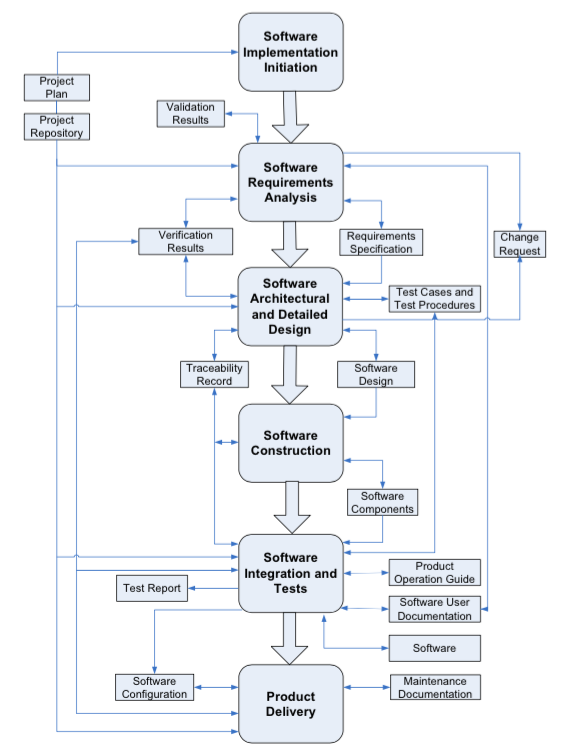
\includegraphics[scale=0.5]{figuras/dsw_diagr.png}
\caption{Diagrama do processo de \dsw \cite[pág. 30]{iso}}
\label{fig:dsw:diagr}
\end{figure}

